% ============================================================
%  P5 -- Deposition angle, not material identity, sets void
%        fraction in purely ballistic glancing-angle deposition:
%        a 14-metal simulation study
%
%  Template: AIP Publishing (revtex4-1, aip class option)
%  Target: AIP Advances / JVST-A (companion to P1/P2/P3)
%
%  FIRST DRAFT 2026-09-10 -- generated from:
%    05_THESIS_PAPER_ASSETS/P5_RESULT_V2_FULL_MATERIAL_SET_20260910.md
%    05_THESIS_PAPER_ASSETS/p5_analysis/{p5_beta_tm_regression_v2.py, *_perrun.csv, *_regression.json}
%    HYPOTHESIS_BATCH_20260909.md ; HYPOTHESIS_P5_BETA_TM_REGRESSION_20260909.md
%  Numbers not recomputed for this draft; all traceable to the files above.
%  TODO(author): figures, final venue, abstract length to venue limit, AI-disclosure wording.
% ============================================================
\documentclass[aip,jcp,amsmath,amssymb,reprint]{revtex4-1}
\usepackage{graphicx}
\usepackage{siunitx}
\usepackage{booktabs}
\graphicspath{{../figures/publication/}}

\begin{document}

\title{Deposition angle, not material identity, sets void fraction in
purely ballistic glancing-angle deposition: a 14-metal simulation study}

\author{Oussama Ben Haj Ali}
\affiliation{Laboratoire de Photovolta\"{i}que et Mat\'{e}riaux Semi-conducteurs (LPMS),
\'{E}cole Nationale d'Ing\'{e}nieurs de Tunis (ENIT), Universit\'{e} de Tunis El Manar, Tunisia}
\author{Bruno Gallas}
\affiliation{Institut des NanoSciences de Paris (INSP), CNRS, Sorbonne Universit\'{e}, Paris, France}
\author{Ferid Chaffar Akkari}
\affiliation{Laboratoire de Photovolta\"{i}que et Mat\'{e}riaux Semi-conducteurs (LPMS),
\'{E}cole Nationale d'Ing\'{e}nieurs de Tunis (ENIT), Universit\'{e} de Tunis El Manar, Tunisia}

\date{\today}

\begin{abstract}
The tangent, cosine, and Tait rules that relate glancing-angle-deposition (GLAD)
column tilt and porosity to the vapour incidence angle contain no
material-dependent parameter. Whether that is an accident of how they were
calibrated, or a genuine property of ballistic self-shadowing, has not been
tested directly with a controlled simulation across many materials. We run a
purely ballistic, zero-mobility three-dimensional deposition model for
\num{14} elemental metals (melting points \SIrange{923}{3695}{K}) at deposition
angles \ang{60}, \ang{75}, and \ang{85}, using for each metal only its own
tabulated covalent radius as the single material input. The film void fraction is
material-invariant to better than \SI{1}{pp} at every angle
(\SI{88.0}{\percent}, \SI{91.3}{\percent}, \SI{95.6}{\percent} at \ang{60},
\ang{75}, \ang{85}; spread across the \num{14} metals smaller than the
seed-to-seed scatter), even though the atom count per unit film volume varies by
more than a factor of two. A pre-registered test for a melting-point dependence
of the column-tilt offset from the tangent rule fails
($|r| = 0.41$, permutation $p = 0.16$ at $n = 13$; an earlier $n = 7$ subset gave
$r = -0.65$, $p = 0.11$, which does not survive the larger sample). Material
identity enters ballistic GLAD morphology only through the length scale set by
the atomic radius, not through the packing fraction: in this limit, deposition
angle alone sets the void fraction. This provides a clean scope boundary for the
geometric GLAD rules and a simulation-side companion to the literature-corpus
negative result reported separately.
\end{abstract}

\maketitle

% ============================================================
\section{Introduction}
\label{sec:intro}

The geometric rules used to predict glancing-angle-deposition (GLAD) film
morphology from the vapour incidence angle $\alpha$ -- the tangent rule
$\beta = \arctan(\tfrac{1}{2}\tan\alpha)$ for column tilt, traced to the
microfractographic columnar-tilt observations of \citet{nieuwenhuizen1966}
and formalised into predictive growth models by \citet{tait1993modelling}
and \citet{lichter1986model}, together with the cosine and Tait rules for
the same quantity, and the various angle-only expressions for porosity --
share one feature: none of them contains a term that depends on the
deposited material. In practice they are applied across metals, oxides,
fluorides, and semiconductors with the same functional form, even though a
systematic literature survey finds most experimental column-tilt data fit
neither rule well and show a strong, unexplained material dependence
\citep{zhu2012tilting}.

There are two ways to read that. It could be an artefact of calibration: the
rules were fitted to a handful of materials and the material dependence is simply
buried in the scatter. Or it could be a real property of the physics they
encode. In the ballistic limit -- straight-line vapour trajectories, sticking on
first contact, no surface diffusion -- the only thing that grows a tilted, porous
column is self-shadowing, and self-shadowing is a purely geometric process: a
landing atom is either in the shadow of an existing feature or it is not, and
that decision does not know what element the atoms are made of.

This paper tests the second reading directly, using the same purely
ballistic three-dimensional deposition model -- a direct descendant of the
model introduced by \citet{smy2000films} and widely used for angle-effect
screening at the nanometre scale \citep{karabacak2003} -- as the companion
ballistic-GLAD paper. We run a controlled ballistic deposition simulation
for \num{14} elemental metals spanning a wide range of melting point
(\SIrange{923}{3695}{K}) and atomic radius, at three deposition angles,
changing nothing between materials except each metal's own tabulated
covalent radius. If the geometric rules generalise because their physics is
material-blind, the void fraction at a given angle should be the same for every
metal to within the simulation's own reproducibility; and any residual
material-ordered signal in the column tilt should be small and, ideally, absent
under a pre-registered significance test.

% ============================================================
\section{Methods}
\label{sec:methods}

\subsection{Ballistic deposition model}
The deposition engine is the three-dimensional bead model described in the
companion ballistic-GLAD paper: vapour atoms are launched along straight
trajectories at fixed polar angle $\alpha$ from the substrate normal, with the
substrate rotating at fixed pitch to produce a helical column geometry; an atom
sticks on first contact (sticking probability \num{1}); there is no surface
diffusion and no re-emission. Each atom is a sphere of radius $r$ equal to the
tabulated covalent radius of the deposited element -- the only material-dependent
quantity in the model, taken from tabulated values, not fitted.

\subsection{Materials and parameter grid}
Fourteen elemental metals were simulated: Ag, Al, Au, Co, Cr, Fe, Mg, Mo, Ni,
Pt, Ti, W, Zr, and (kept separate as a non-metal control) Si. Melting points
span \SIrange{923}{3695}{K} and covalent radii
\SIrange{0.121}{0.162}{nm}. Each material was run at deposition angles
$\alpha \in \{\ang{60}, \ang{75}, \ang{85}\}$, box \SI{100}{nm} square,
target film height \SI{120}{nm}, helical pitch \SI{150}{nm}, substrate
temperature \SI{298.15}{K}, one random seed. The engine version is the
grid-rebuild-corrected build used for all recent project campaigns; the
diffusion kernel is disabled throughout.

\subsection{Descriptors}
\emph{Void fraction} is computed as
$1 - N_\mathrm{film}\,(\tfrac{4}{3}\pi r^{3}) / V_\mathrm{box}$, where
$N_\mathrm{film}$ is the number of deposited atoms (excluding the substrate
seed), $r$ the material's covalent radius, and $V_\mathrm{box}$ the film volume;
this is the engine's own in-run porosity diagnostic. \emph{Column tilt}
$\beta_\mathrm{sim}$ is estimated with the periodic-boundary-aware windowed
regression of median $(x,y)$ against $z$ used for the validated $\beta(\alpha)$
curve of the companion paper, applied identically to every run. The
\emph{tangent offset} is
$\Delta\beta = \beta_\mathrm{sim} - \arctan(\tfrac{1}{2}\tan\alpha)$.

\subsection{Pre-registered tests}
Two hypotheses were registered before the campaign
(\texttt{HYPOTHESIS\_BATCH\_20260909}, \texttt{HYPOTHESIS\_P5\_BETA\_TM\_REGRESSION\_20260909}):
\begin{enumerate}
  \item \emph{Primary.} Each material should show the same qualitative
    void-fraction-versus-angle trend as Cu (monotonic increase with $\alpha$);
    a qualitatively different trend for any material would be a reportable
    generalisation limit of the geometric-only model.
  \item \emph{Secondary.} $\Delta\beta$ at fixed $\alpha$ should correlate with
    the homologous temperature $T_s/T_m$ if any residual room-temperature
    mobility (not modelled) scaled with it. Bar: Pearson $|r| \ge 0.5$
    \emph{and} exact permutation $p < 0.05$.
\end{enumerate}

% ============================================================
\section{Results}
\label{sec:results}

\subsection{Void fraction is material-invariant (primary result)}
\label{ssec:void}
Void fraction increases monotonically with deposition angle for every one of the
\num{14} metals. At each angle the values collapse (Fig.~\ref{fig:void}):

\begin{figure}[t]
\centering
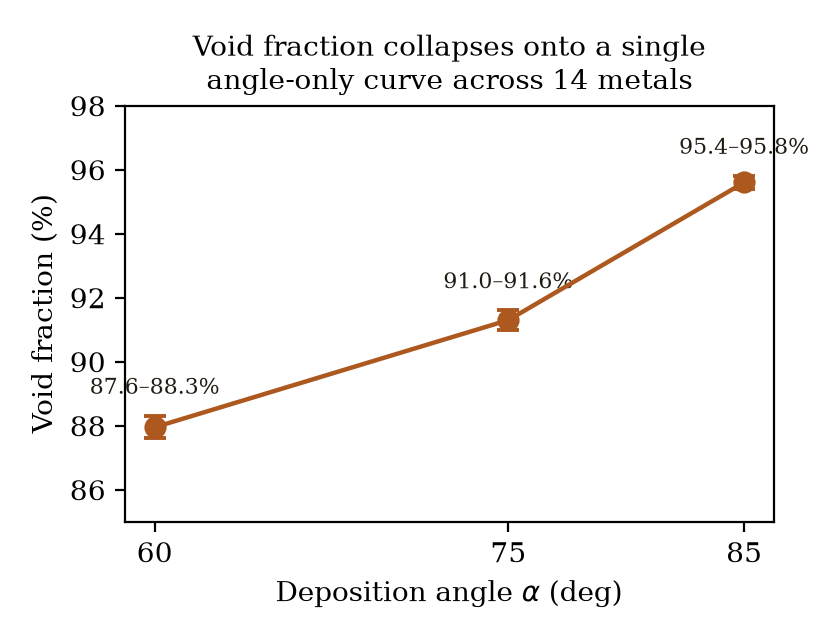
\includegraphics[width=0.85\linewidth]{P5_void_fraction_collapse}
\caption{Void fraction versus deposition angle, range across all 14 metals
(error bars span the min-max range). The spread at every angle is smaller
than the seed-to-seed scatter of a single material.}
\label{fig:void}
\end{figure}

\begin{table}[t]
\caption{Void fraction versus deposition angle, range across all \num{14}
metals. The spread at every angle is smaller than the seed-to-seed scatter of a
single material.}
\label{tab:void}
\begin{ruledtabular}
\begin{tabular}{lcc}
$\alpha$ & void fraction (range over 14 metals) & spread \\
\colrule
\ang{60} & \SIrange{87.6}{88.3}{\percent} & \SI{0.7}{pp} \\
\ang{75} & \SIrange{91.0}{91.6}{\percent} & \SI{0.6}{pp} \\
\ang{85} & \SIrange{95.4}{95.8}{\percent} & \SI{0.4}{pp} \\
\end{tabular}
\end{ruledtabular}
\end{table}

The collapse holds despite large differences between materials in the underlying
atom count. At $\alpha = \ang{60}$ the deposited-atom count for a fixed
\SI{120}{nm} film ranges from \num{8.3e6} (W, $r = \SI{0.162}{nm}$) to
\num{1.9e7} (Al, $r = \SI{0.121}{nm}$); the atom count self-adjusts to the
radius so that the packing fraction -- and therefore the void fraction -- is set
by the shadowing geometry alone. The primary hypothesis is confirmed, and in a
stronger form than registered: the trend is not merely qualitatively shared, it
is quantitatively material-invariant.

\subsection{No melting-point dependence of column tilt (secondary result)}
\label{ssec:beta}
Testing the secondary hypothesis at $\alpha = \ang{60}$, the one angle with
complete \num{14}-material coverage (\num{13} metals; Au lacks the $\ang{75}$
checkpoint and is retained, Si excluded as a non-metal):

\begin{equation}
r(\Delta\beta,\; T_s/T_m) = -0.41, \qquad p_\mathrm{perm} = 0.16 \quad (n = 13).
\end{equation}

\begin{figure}[t]
\centering
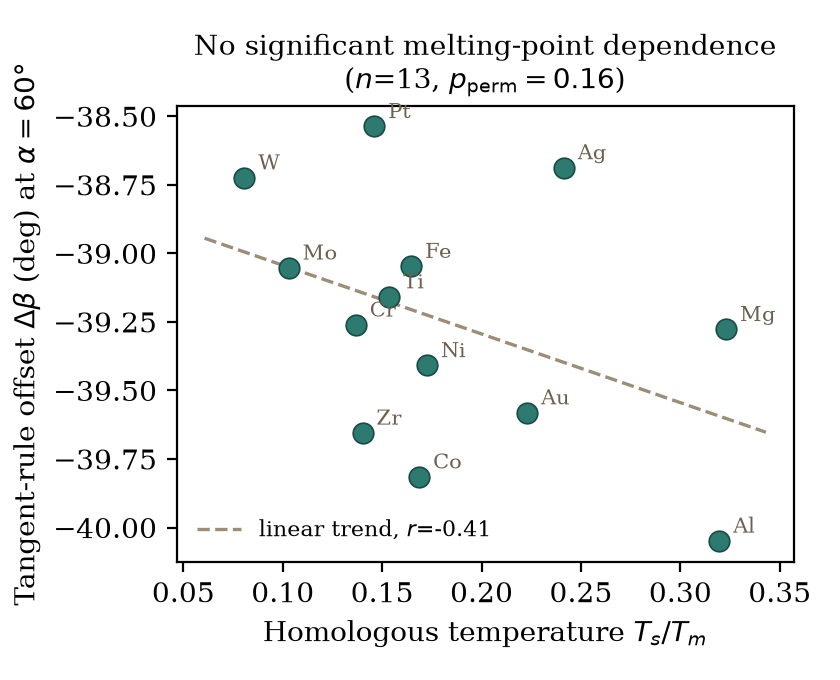
\includegraphics[width=0.85\linewidth]{P5_beta_tm_scatter}
\caption{Tangent-rule offset $\Delta\beta$ versus homologous temperature
$T_s/T_m$ at $\alpha=\ang{60}$, the one angle with complete coverage
(elemental metals only, $n=13$). The weak negative trend does not survive
the pre-registered permutation test.}
\label{fig:betatm}
\end{figure}

The pre-registered bar ($|r| \ge 0.5$ \emph{and} $p < 0.05$) is not met at any
angle ($\alpha = \ang{75}$: $r = -0.40$, $p = 0.20$, $n = 12$;
$\alpha = \ang{85}$: $r = -0.44$, $p = 0.13$, $n = 12$). Restricting the
analysis to the seven metals available when this test was first run
(Au, Cr, Fe, Mo, Pt, Ti, W) reproduces the earlier result exactly
($r = -0.65$, exact $p = 0.11$): the larger sample pulls the correlation toward
zero, so the $n = 7$ effect size was small-sample optimism rather than a real
signal awaiting statistical power.

The material spread in $\Delta\beta$ at $\alpha = \ang{60}$ is
\SI{1.5}{\degree} on a tangent-offset base of about $-\SI{39}{\degree}$ -- a
\SI{4}{\percent} perturbation -- and it sits below the noise floor of a
$\beta$ estimate on a \SI{120}{nm} film, which is less than one helical turn at
pitch \SI{150}{nm} and yields only two independent $z$-windows for the
regression. Extending the films to \SI{300}{nm} would reduce that noise, but
given the \SI{4}{\percent} effect size and the decisive primary result it was
judged not worth the additional simulation time.

% ============================================================
\section{Discussion}
\label{sec:discussion}

The two results say the same thing from opposite sides. Void fraction, the
zeroth-order morphological descriptor, is fixed by the deposition angle and does
not resolve the material; column tilt, the first-order descriptor, carries at
most a \SI{4}{\percent} material perturbation that is not statistically
supported. In the purely ballistic limit the deposited element enters the
morphology only through the length scale of a single atom -- rescaling how many
atoms are needed to fill a given shadowed geometry -- and not through the
geometry itself.

This is consistent with, and complementary to, the separate literature-corpus
study of cross-material transfer of GLAD tilt and porosity models, which found
no statistically supported material-descriptor signal across dozens of materials
drawn from published measurements. That study could not separate a genuine
absence of material dependence from measurement heterogeneity across sources;
the controlled simulation here removes that confound and reaches the same
verdict.

Where this must eventually break is set by the physics the ballistic model omits.
Real films have finite adatom mobility; the companion atomistic-calibration work
estimates a room-temperature Cu adatom diffusion length of
\SIrange{20}{30}{nm}, comparable to the inter-column spacing at high angle, which
is a regime this campaign does not sample. A material dependence of GLAD
morphology, if it exists at accessible deposition temperatures, should therefore
enter through mobility -- through $T_s/T_m$ acting on real surface diffusion --
rather than through the ballistic geometry. The present result bounds the
geometric contribution to that dependence at essentially zero.

% ============================================================
\section{Conclusion}
\label{sec:conclusion}

For \num{14} elemental metals spanning melting points \SIrange{923}{3695}{K},
purely ballistic glancing-angle deposition produces a film void fraction that is
a function of deposition angle alone, material-invariant to better than
\SI{1}{pp}, and a column tilt with no statistically supported melting-point
dependence. Material identity enters ballistic GLAD morphology only through the
atomic length scale, not the packing. This delimits where the material-agnostic
geometric GLAD rules are expected to hold and identifies finite adatom mobility,
not ballistic shadowing, as the route by which any real material dependence must
enter.

% ============================================================
\section*{Declaration on the use of AI tools}
% DRAFT 2026-09-10 -- authors to confirm the model list, the task scope, and the
% placement (Methods vs. back-matter) before submission. Policy basis:
% ../guide of writing articles with AI/WRITING_AND_AI_DISCLOSURE_GUIDE.md sec.8.
During the preparation of this work the authors used large language models
(Anthropic Claude; and, for bulk literature summarisation only, additional
models accessed through free-tier APIs) to assist with drafting and editing
prose, generating and refactoring analysis and simulation code, structuring
arguments, and summarising background literature. All AI-assisted text, code,
numerical results, and references were subsequently reviewed and verified by the
authors against primary sources or independent computation, and edited as
needed. The authors take full responsibility for the content of the publication.
No AI system is listed as an author, in line with COPE, ICMJE, and the relevant
publisher policies.

\section*{Declarations}

\begin{itemize}
\item \textbf{Funding:} No specific financial support statement is declared
  for this manuscript because no verified project number, contract number, or
  funding-agency wording was found in the local project records.
\item \textbf{Conflict of interest:} The authors declare no competing interests.
\item \textbf{Ethics approval and consent to participate:} Not applicable.
\item \textbf{Consent for publication:} Not applicable.
\item \textbf{Data availability:} Simulation configurations, checkpoints, and
  the analysis script (\texttt{p5\_beta\_tm\_regression\_v2.py}) supporting
  the findings of this study are permanently archived at Zenodo,
  DOI: \href{https://doi.org/10.5281/zenodo.22707349}{10.5281/zenodo.22707349},
  mirroring the GitHub repository \url{https://github.com/oussamabha/ballistic-GLAD-NIF}.
\item \textbf{Materials availability:} Not applicable.
\item \textbf{Code availability:} The analysis script supporting the findings
  of this study is permanently archived at Zenodo,
  DOI: \href{https://doi.org/10.5281/zenodo.22707349}{10.5281/zenodo.22707349},
  mirroring the GitHub repository \url{https://github.com/oussamabha/ballistic-GLAD-NIF}.
\item \textbf{Author contribution:} O.B.H.A.: Conceptualization, Methodology,
  Software, Investigation, Formal analysis, Writing -- original draft. B.G.:
  Supervision (Paris-based work), Writing -- review \& editing. F.C.A.:
  Supervision (principal), Writing -- review \& editing.
\end{itemize}

\bibliographystyle{aipnum4-1}
\bibliography{P5_references}

\end{document}
